


\section{Complex Power }
\subsection{2 examples of Complex Power}

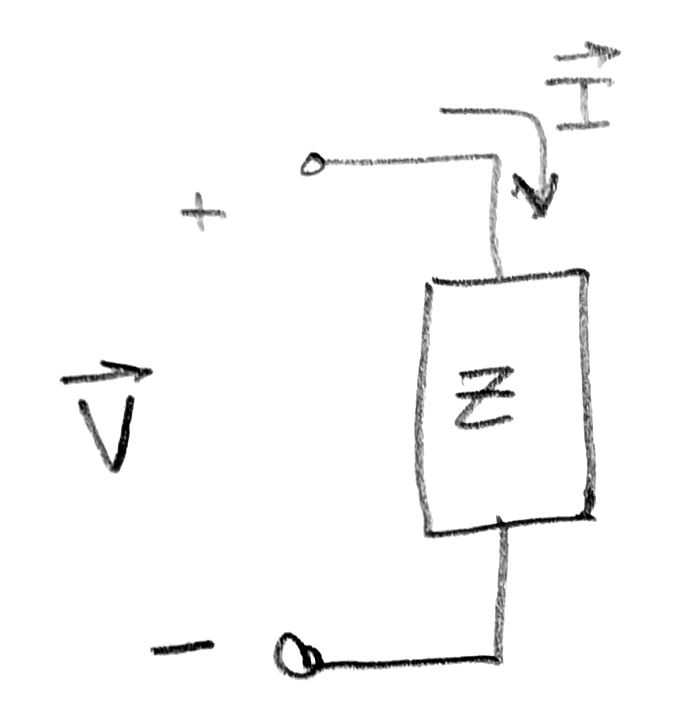
\includegraphics[width=0.3\textwidth]{MB87549.png}


1)
\[
 \quad S = \vec{V} \vec{I}^*,
\]
and
\[ \vec{I}^* = \frac{\vec{V}^*}{\vec{Z}^*}
\]

so
\[
S = \frac{\vec{V} \vec{V}^*}{\vec{Z}^*} = \frac{|\vec{V}|^2}{\vec{Z}^*} = \frac{V^2}{\vec{Z}^*}
\]

2)
\[
 \quad \vec{V} = \vec{I} \vec{Z}
\]

\[
S = \frac{\vec{I} \vec{I}^* \vec{Z}}{\vec{Z}}
\]

\[
= |\vec{I}|^2 \vec{Z} = I^2 \vec{Z} = \frac{I_M^2}{2} \vec{Z}
\]


\begin{itemize}
\item In both cases, $\angle S = \angle Z$

\item RMS current and voltage phasors can be used like DC voltage and current where

$R \rightarrow \vec{Z}$

$A^2 \rightarrow A A^* = |A|^2$
\end{itemize}

e.g.

\begin{center}
\begin{tabular}{c|c}
DC & RMS \\
\hline
$P = I^2 R$ & $S = |\vec{I}_R|^2 \vec{Z}$ \\
$P = \frac{V^2}{R}$ & $S = \frac{|\vec{V}_R|^2}{\vec{Z}^*}$ \\
\end{tabular}
\end{center}

\newpage

\subsection{Conservation of Complex Power}

\noindent Consider

%\includegraphics[width=0.4\textwidth]{(see Chapt02 parallel Zs).png}

by KCL, (+ current leaving node (A))

\[
-\vec{I}_R + \vec{I}_{R_1} + \vec{I}_{R_2} = 0
\]


\[
-\vec{I} + \vec{I}_1 + \frac{\vec{I}_2}{V_2} = 0
\]

\[
-i_{R_1} + i_1(t) + i_2(t) = 0
\]

etc.

\[
\vec{I}_R = \vec{I}_{R_1} + \vec{I}_{R_2}
\]

\[
S = \vec{V} \vec{I}_R^* = \vec{V}_R (\vec{I}_{R_1}^* + \vec{I}_{R_2}^*)
\]

\[
= S_1 + S_2
\]

\noindent Also:

%\includegraphics[width=0.4\textwidth]{series_circuit.png}



\noindent Also consider

%\includegraphics[width=0.4\textwidth]{Chapt02 voltage div ckt.png}

Using KVL

\[
-\vec{V}_R + \vec{V}_{1R} + \vec{V}_{2R} = 0
\]

\[
\Rightarrow \vec{V}_R = V_{1R} + V_{2R}
\]

\[
S = \vec{V}_R \vec{I}_R^* = (\vec{V}_{1R} + \vec{V}_{2R}) \vec{I}_R^*
\]

\[
= S_1 + S_2
\]

Thus, complex power in whole circuit can be obtained by adding complex power in each Z.


\newpage
\section{Application: Power Factor Correction}


%\includegraphics[width=0.5\textwidth]{transmission_line.png}

\noindent We know
\[
P_{AV_{\text{user}}} = \text{Re}\{S_{\text{user}}\} ??????????
\]

\[
P_{\text{plant}} = \text{Re}\{S_{\text{user}}\} + |\vec{I}_R|^2 R
\]

\hspace{5cm} loss in lines

\hspace{5cm} want to reduce

\noindent Consider $\vec{Z}_L = R + jX$ (typ $X > 0$: inductive)

aka positive etc.)

\[
\Theta > 0
\]
\[
pf < 1
\]

\[
P_{AV_{\text{user}}} = \text{Re}\left\{ |\vec{I}_R|^2 \vec{Z}_L \right\}
\]

\[
= \text{Re}\left\{ |\vec{I}_R| |\vec{Z}_L| (\cos \angle z_L + j \sin \angle z_L) \right\}
\]

\[
= |\vec{I}_R| |\vec{Z}_L| \cos \angle z_L = P
\]

\noindent Assume constant power use, P. Note: Loss proportional to $|\vec{I}_R|^2$, so how does $\vec{I}_R$ depend on pf of $z_L$?

\[
|\vec{I}_R|^2 = \frac{P}{|\vec{Z}_L| \cos \angle z_L}
\]

\noindent i.e. for fixed P, $z_L$, loss $|\vec{I}_R|^2 R$ is minimized when $\cos \angle z_L = 1$


\noindent Can thus remove losses by ``correcting pf''

Ex

%\includegraphics[width=0.4\textwidth]{pf_correction.png}

\[
\vec{Z}_L = R + j\omega L
\]
\[
S = P + jQ_L
\]

(Receive power)

%\includegraphics[width=0.3\textwidth]{power_triangle.png}

\noindent Could use series C but

if we add C in parallel,

\[
S = S_C + S_{ZL}
\]

%\includegraphics[width=0.3\textwidth]{phasor_diagram2.png}

\noindent Can be shown that (problem $\cos(\phi)$)

\[
C = \frac{Q_L - P \tan \Theta_1}{\sqrt{|\vec{V}_R|^2} \omega}
\]

\hspace{4cm} look at pg 485


\noindent Problem 12.2.2

%\includegraphics[width=0.5\textwidth]{problem_circuit.png}

\[
< z_{TH}
\]

\[
P_{AV_{\text{Source}}} = P_{AV_{AC}} + P_{AV_{DC}}
\]
%
% by superposition of power
%
% at diff freq

\[
= \left\{ \text{Re}\{\vec{V}_{2R} \vec{I}_{2R}^*\} \right\} + \frac{2\pi}{T} \int_0^{2\pi/T} \left\{ 50 \cdot 0.1 \cos(1000t) \right\} dt
\]

\noindent For part SOURCE

\[
= -\text{Re}\left\{ \vec{I}_{2R} \vec{Z}_{TH} \vec{I}_{2R}^* \right\} + \frac{10}{1000} \int_0^{1000/2\pi} \left( \cos(1000)dt \right)
\]

\[
= -\text{Re}\left\{ |\vec{I}_{2R}|^2 \vec{Z}_{TH} \right\}
\]

\hspace{5cm} 0

\[
\vec{Z}_{TH} = 500 \parallel -j1000 = 400 - 200j
\]

\[
P_{AV_{\text{Source}}} = -\text{Re}\left\{ 0.005(400 + 200j) \right\}
\]

\[
= -2 \text{ Watts } //
\]



\section{Power Meters}

%\includegraphics[width=0.4\textwidth]{meter_circuit.png}

\noindent Meter doesn't effect circuit thus

\[
\vec{Z}_{cc} = 0
\]
\[
\vec{Z}_{vc} = \infty
\]

\noindent $\circ$ Indicates polarity for positive power reading when power is absorbed by $\vec{Z}_L$.

\noindent Two coils drive the disk. Where velocity $\propto$ real power gears integrate velocity to dial positions.

\[
V_{disk} \propto V_R I_R \cos \angle z_L \cdot c
\]

\[
C = -\frac{1}{\omega T} \text{ if } | \text{ coil is reversed}
\]

wrt $\bullet$


\subsection*{Ex}

%\includegraphics[width=0.5\textwidth]{meter_example.png}

\noindent Q: What will meter read?

\[
A: \quad \vec{I}_R = \frac{\vec{V}_R}{\vec{Z}_1 + \vec{Z}_2} \quad |\vec{I}_R| = \frac{|\vec{V}_R|}{|\vec{Z}_1 + \vec{Z}_2|}
\]

\[
\vec{V}_{2R} = \vec{I}_R \vec{Z}_2 = \frac{\vec{Z}_2 \vec{V}_R}{\vec{Z}_1 + \vec{Z}_2}
\]

\[
P_{\text{meter}} = |\vec{I}_R| |\vec{V}_{2R}| \cos \angle z_2
\]

\[
= \frac{|\vec{V}_R| |\vec{V}_R| |\vec{Z}_2|}{|\vec{Z}_1 + \vec{Z}_2|^2} \cos \angle z_2
\]

\[
= \frac{|\vec{V}_R|^2 |\vec{Z}_2|}{|\vec{Z}_1 + \vec{Z}_2|^2} \cos \angle z_2
\]
